%%% License: Creative Commons Attribution Share Alike 4.0 (see https://creativecommons.org/licenses/by-sa/4.0/)
%%% Slides are based heavily on earlier versions of this course taught by Jesper Rudiger.

%%% License: Creative Commons Attribution Share Alike 4.0 (see https://creativecommons.org/licenses/by-sa/4.0/)
%%% Slides are based heavily on earlier versions of this course taught by Jesper Rudiger and Peter Norman Sorensen.

\DeclareGraphicsExtensions{.eps, .pdf,.png,.jpg,.mps,}
\usetheme{reMedian}
\usepackage{parskip}
\makeatother

\renewcommand{\baselinestretch}{1.1} 

\usepackage{amsmath, amssymb, amsfonts, amsthm}
\usepackage{enumerate}
\usepackage{hyperref}
\usepackage{url}
\usepackage{bbm}
\usepackage{color}

\usepackage{tikz}
\usepackage{tikzscale}
\newcommand*\circled[1]{\tikz[baseline=(char.base)]{
		\node[shape=circle,draw, inner sep=-20pt] (char) {#1};}}
\usetikzlibrary{automata,positioning}
\usetikzlibrary{decorations.pathreplacing}
\usepackage{pgfplots}
\usepgfplotslibrary{fillbetween}
\usepackage{graphicx}

\usepackage{setspace}
%\thinmuskip=1mu
%\medmuskip=1mu 
%\thickmuskip=1mu 


\usecolortheme{default}
\usepackage{verbatim}
\usepackage[normalem]{ulem}

\usepackage{apptools}
\AtAppendix{
	\setbeamertemplate{frame numbering}[none]
}
\usepackage{natbib}




\title{Financial Markets Microstructure \\ Exercise class 1}

\author{Egor Starkov}

\date{K{\o}benhavns Unversitet \\
	Spring 2020}



\begin{document}
\frame[plain]{\titlepage}
\addtocounter{framenumber}{-1}



\section{Strategic vs Competitive behavior}

\begin{frame}{Problem 0}
	(Related to Lecture 1, not stated in the slides:)
	
	How does \alert{strategic} behavior differ from \structure{competitive behavior}?
\end{frame}


\begin{frame}{Price-taking behavior (`thruthful' bidding)}
	Suppose the possible prices are $\{1,2,3,4,5\}$. At these prices:
	\begin{itemize}
		\item Agent 1 will supply respectively 2, 3, 5, 6, 8
		\item Agent 2 will demand respectively 10, 7, 7, 6, 4
	\end{itemize}
	\begin{figure}
		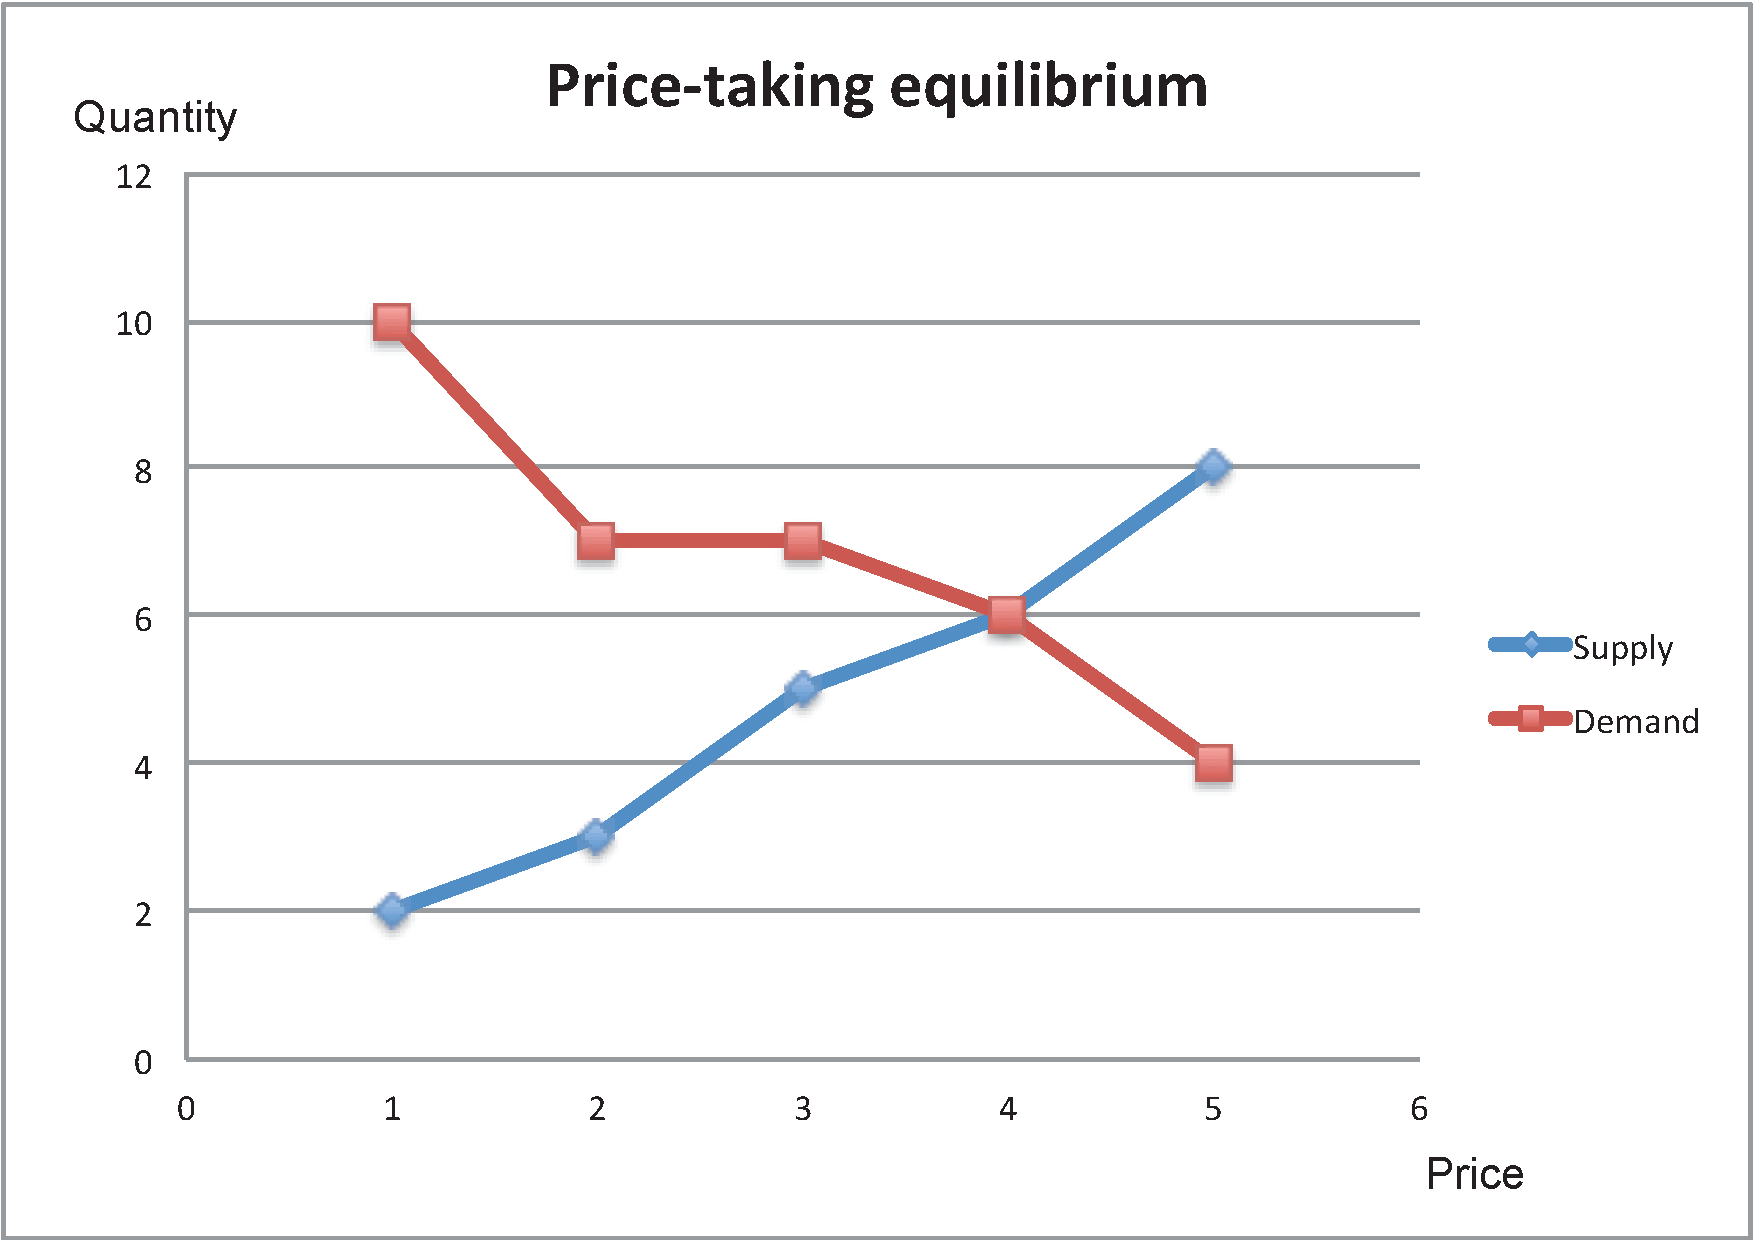
\includegraphics[width=.4\paperwidth]{pics/Image_PriceTaking2}
	\end{figure}
	Here: agents truthfully state their demand/supply
\end{frame}


\begin{frame}{Strategic bidding}
	\begin{itemize}
		\item What if agent 2 prefers 5 units at price 3 instead of 6 units at price 4?
		\item He can 'lie' about his demand schedule to the auctioneer
		\item Suppose he says he demands 10, 7, 5, 5, 4
	\end{itemize}
	\begin{figure}
		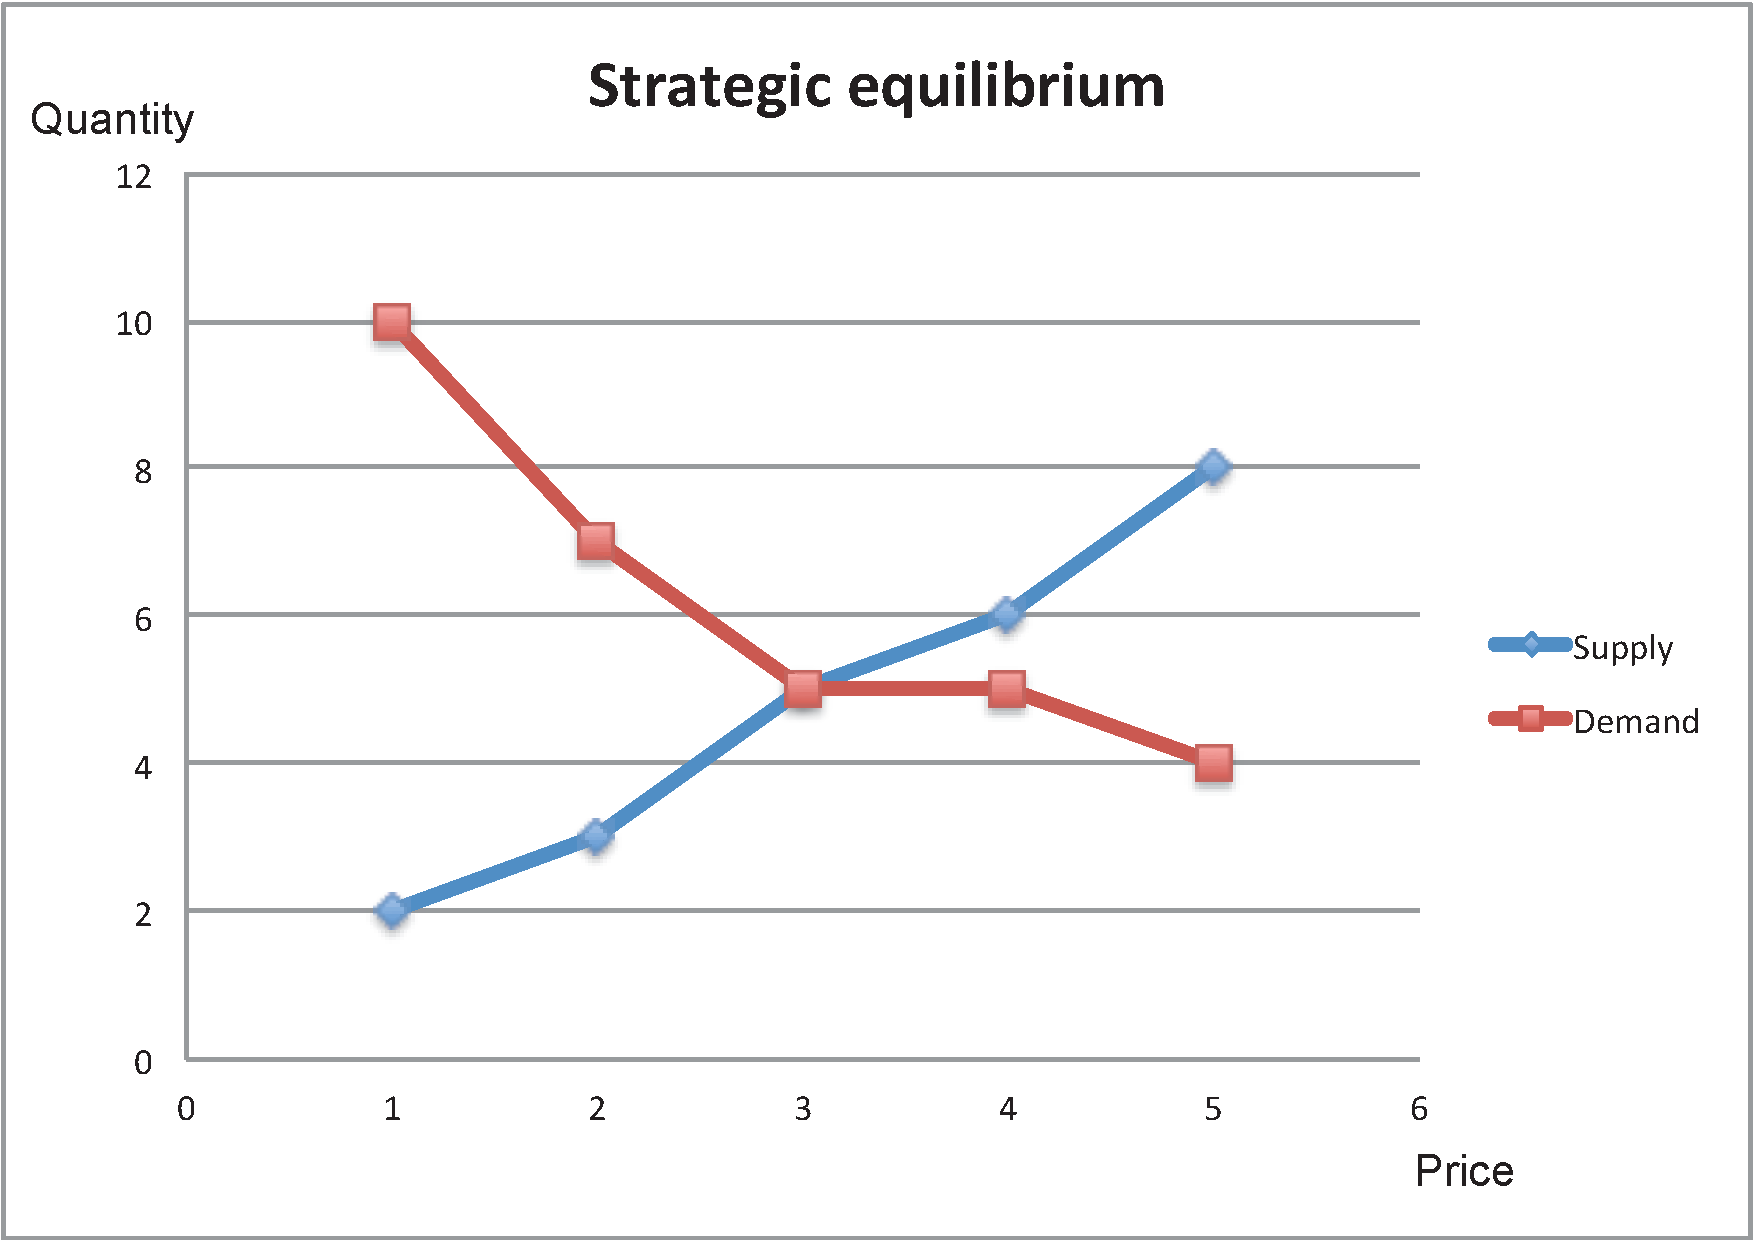
\includegraphics[width=.4\paperwidth]{pics/Image_Strategic2}
	\end{figure}
	Why would agent 2 want fewer units? Pay lower price on all units. (Parallel to monopolist restricting supply to get higher price). \hyperlink{main2}{\beamerbutton{back}}
\end{frame}



\section{Problems from Lecture 1}

\begin{frame}{Lecture 1}
	From Lecture 1: problems 1-3 from FPR ch.1 (pp. 44-45)
\end{frame}


\begin{frame}{Orders}
	We have a collection of limit orders and market orders
	\begin{itemize}
		\item Limit buy orders:
		\begin{itemize}
			\item 100 shares at bid price 3
			\item 200 shares at bid price 4
			\item 200 shares at bid price 3.5
			\item 500 shares at bid price 2.5
		\end{itemize}
		\item Limit sell orders:
		\begin{itemize}
			\item 500 shares at ask price 5
			\item 600 shares at ask price 3
			\item 500 shares at ask price 4
		\end{itemize}
		\item Market buy order: 500
		\item Market sell order: 200
	\end{itemize}
\end{frame}


\begin{frame}{Call auction}
	Recall idea of a call auction:
	\begin{itemize}
		\item Orders are collected (in a `batch') and cleared at a certain frequency
		\item The price is chosen so as to maximize the number of executed orders
		\item \textcolor{red}{Uniform price}: all orders in a batch trades at same price
	\end{itemize}
	\quad
	Let's build the auction step by step
\end{frame}


\begin{frame}{Call auction}
	Limit buy order of 100 shares at bid price 3
	\quad
	\center
	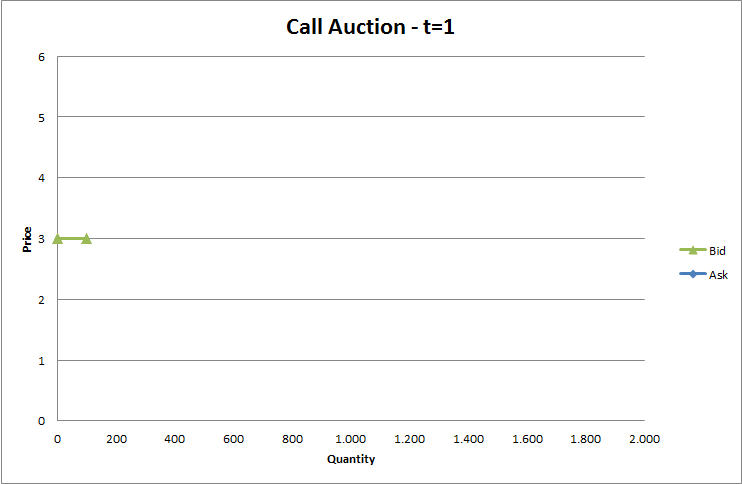
\includegraphics[width=.75\linewidth]{pics/Call_t1}
\end{frame}


\begin{frame}{Call auction}
	Limit buy order of 200 shares at bid price 4
	\quad
	\center
	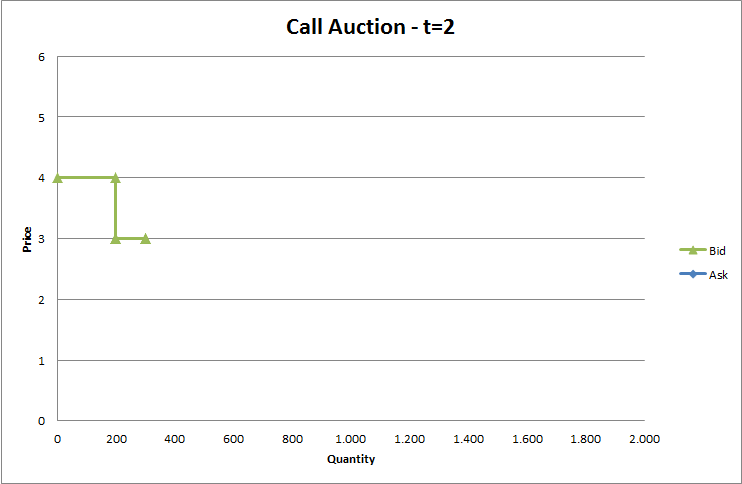
\includegraphics[width=.75\linewidth]{pics/Call_t2}
\end{frame}


\begin{frame}{Call auction}
	Limit buy order of 200 shares at bid price 3.5
	\quad
	\center
	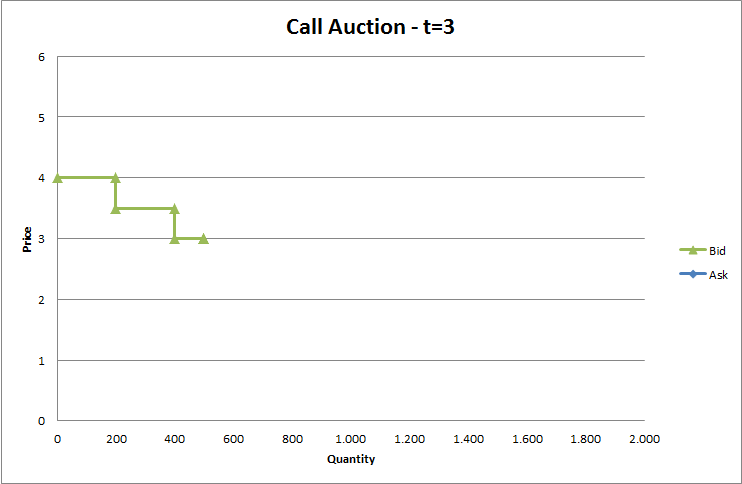
\includegraphics[width=.75\linewidth]{pics/Call_t3}
\end{frame}


\begin{frame}{Call auction}
	Limit buy order of 500 shares at bid price 2.5
	\quad
	\center
	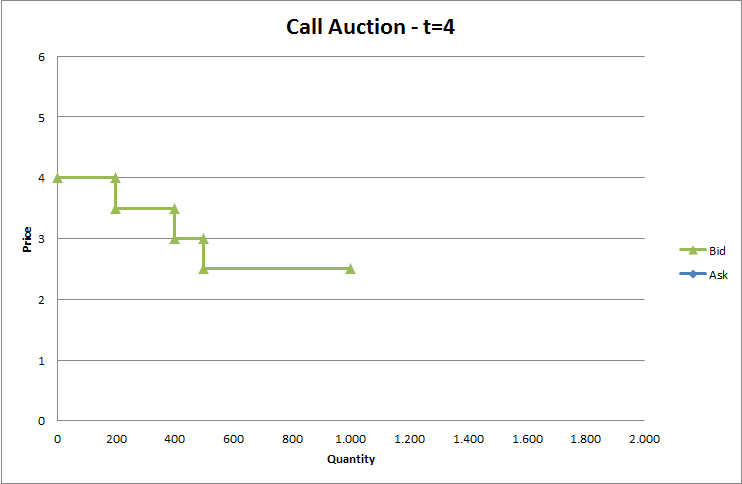
\includegraphics[width=.75\linewidth]{pics/Call_t4}
\end{frame}


\begin{frame}{Call auction}
	Limit sell order of 500 shares at ask price 5
	\quad
	\center
	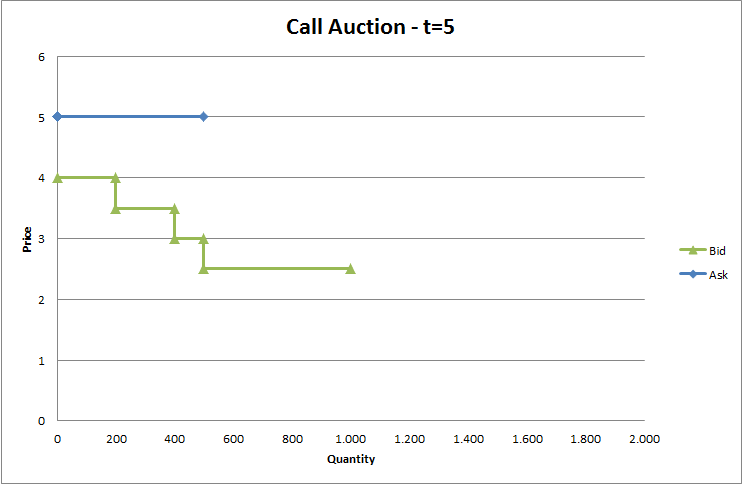
\includegraphics[width=.75\linewidth]{pics/Call_t5}
\end{frame}


\begin{frame}{Call auction}
	Limit sell order of 600 shares at ask price 3
	\quad
	\center
	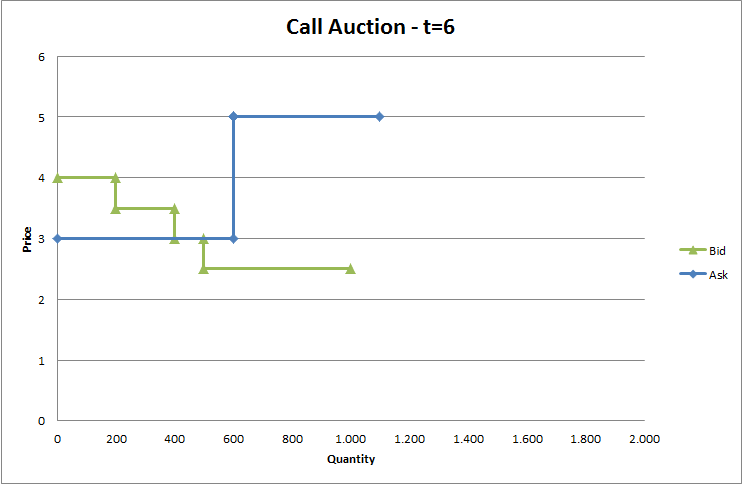
\includegraphics[width=.75\linewidth]{pics/Call_t6}
\end{frame}


\begin{frame}{Call auction}
	Limit sell order of 500 shares at ask price 4
	\quad
	\center
	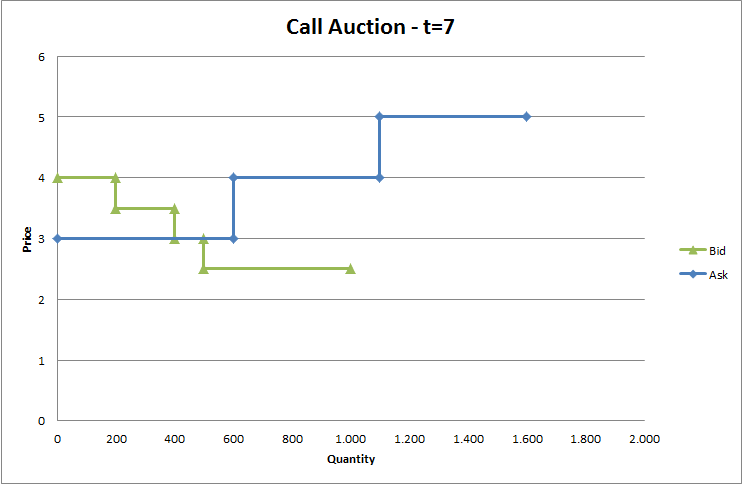
\includegraphics[width=.75\linewidth]{pics/Call_t7}
\end{frame}


\begin{frame}{Call auction}
	Market buy order of 500 shares
	\quad
	\center
	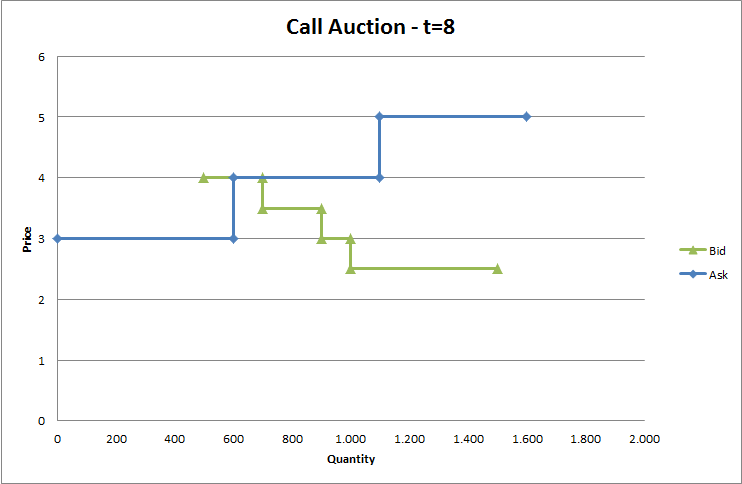
\includegraphics[width=.75\linewidth]{pics/Call_t8}
\end{frame}


\begin{frame}{Call auction}
	Market sell order of 200 shares
	\quad
	\center
	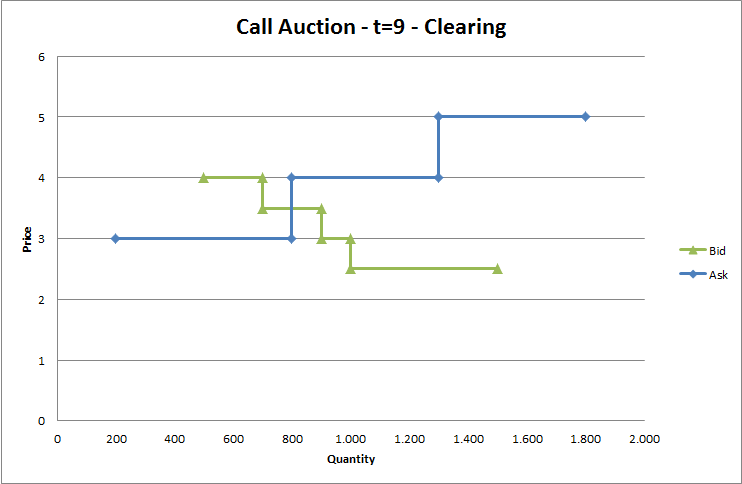
\includegraphics[width=.75\linewidth]{pics/Call_Clearing}
\end{frame}


\begin{frame}{Call auction}
	Market clears at price 3.5, with 800 units being sold
	Filled buy orders:
	\begin{itemize}
		\item The market order is filled completely
		\item The limit order for 200 shares at price 4 is filled completely
		\item The limit order for 200 shares at price 3.5 is filled partially (100 shares)
	\end{itemize}
	Filled sell orders:
	\begin{itemize}
		\item The market order is filled completely
		\item The limit order for 600 shares at price 3 is filled completely
	\end{itemize}
	Thus: \textit{Excess demand} at the clearing price
\end{frame}


\begin{frame}{Continuous auction}
	Recall idea of a continuous auction:
	\begin{itemize}
		\item Some traders post limit orders (provide liquidity)
		\item Some traders post market orders (take liquidity)
		\item Trades occur either through 
		\begin{enumerate}
			\item a limit order 'match' (somebody posts a bid price above the lowest ask price), or
			\item through market orders
		\end{enumerate}
		\item \textcolor{red}{Discriminatory price}: depends on how your order is matched
	\end{itemize}
\end{frame}


\begin{frame}{Continuous auction}
	Limit buy order of 100 shares at bid price 3
	\quad
	\center
	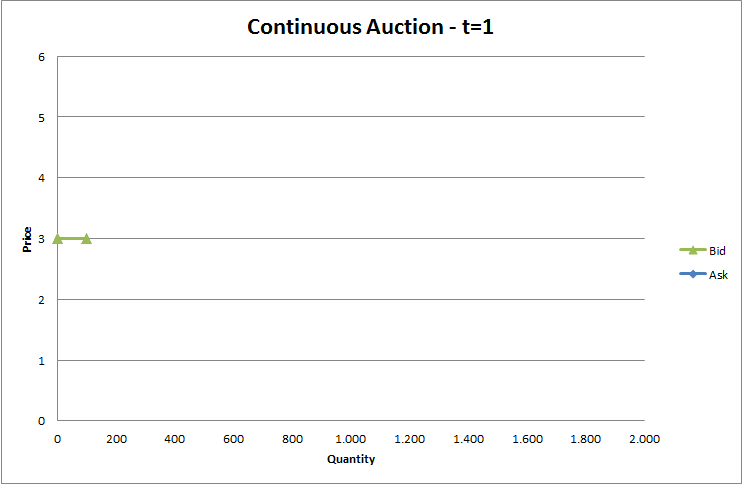
\includegraphics[width=.75\linewidth]{pics/Continuous_t1}
\end{frame}


\begin{frame}{Continuous auction}
	Limit buy order of 200 shares at bid price 4
	\quad
	\center
	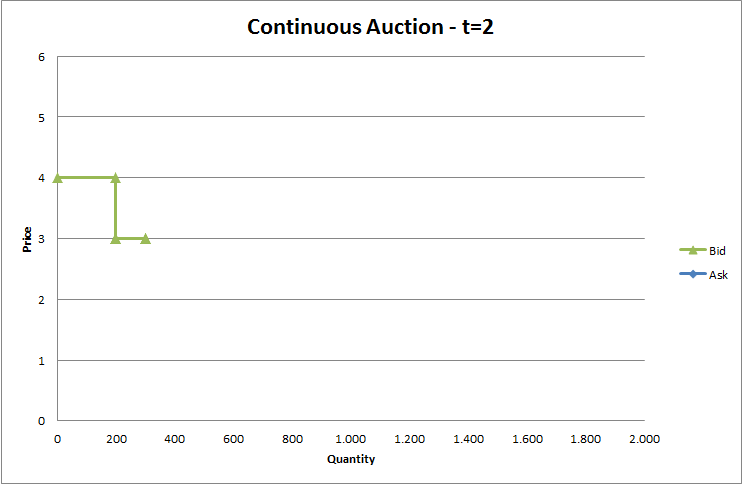
\includegraphics[width=.75\linewidth]{pics/Continuous_t2}
\end{frame}


\begin{frame}{Continuous auction}
	Limit buy order of 200 shares at bid price 3.5
	\quad
	\center
	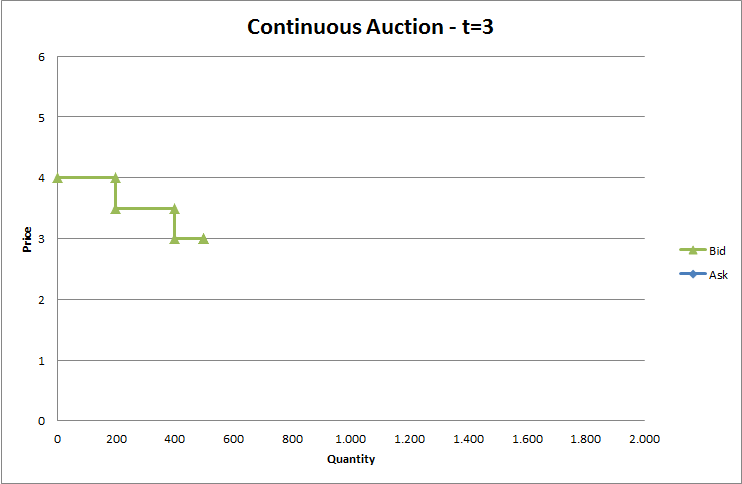
\includegraphics[width=.75\linewidth]{pics/Continuous_t3}
\end{frame}


\begin{frame}{Continuous auction}
	Limit buy order of 500 shares at bid price 2.5
	\quad
	\center
	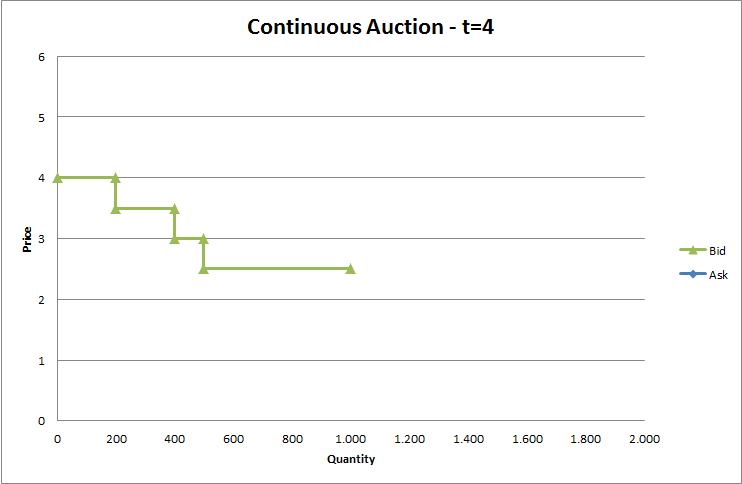
\includegraphics[width=.75\linewidth]{pics/Continuous_t4}
\end{frame}


\begin{frame}{Continuous auction}
	Limit sell order of 500 shares at ask price 5. Spread =  1
	\quad
	\center
	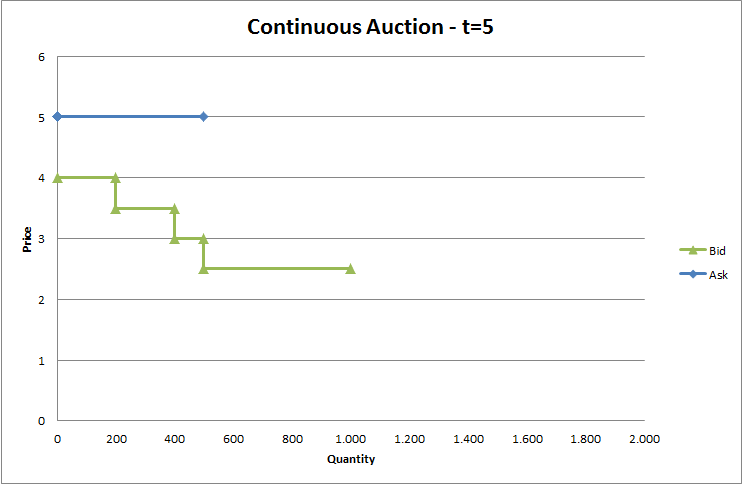
\includegraphics[width=.75\linewidth]{pics/Continuous_t5}
\end{frame}


\begin{frame}{Continuous auction}
	Limit sell order of 600 shares at ask price 3
	\quad
	\center
	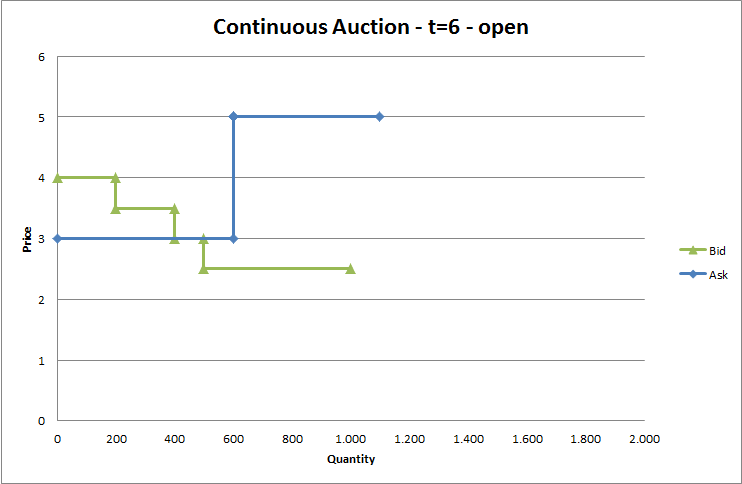
\includegraphics[width=.75\linewidth]{pics/Continuous_t6open}
\end{frame}


\begin{frame}{Continuous auction}
	Seller executes 200 shares at price 4, 200 at price 3.5, and 100 at price 3. Spread = 0.5
	\center
	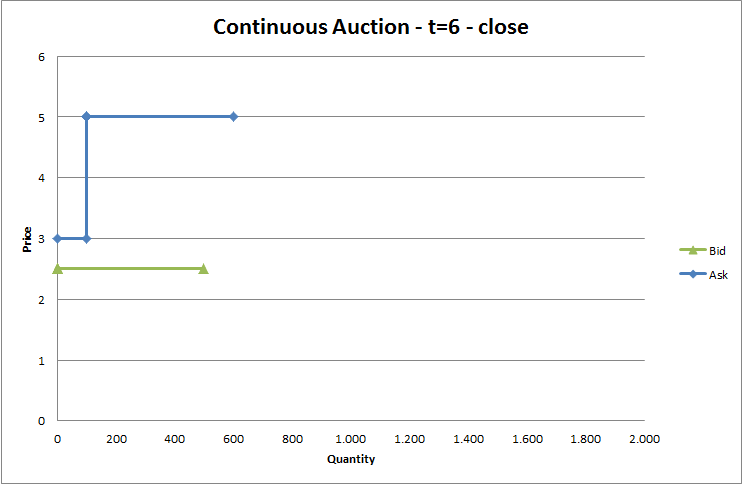
\includegraphics[width=.75\linewidth]{pics/Continuous_t6close}
\end{frame}


\begin{frame}{Continuous auction}
	Limit sell order of 500 shares at ask price 4. Spread = 0.5
	\center
	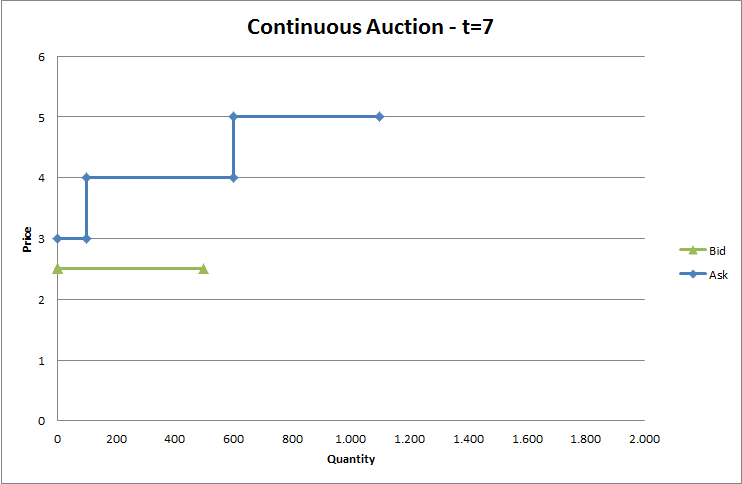
\includegraphics[width=.75\linewidth]{pics/Continuous_t7}
\end{frame}


\begin{frame}{Continuous auction}
	Market buy order of 500 shares. Executes against 100 shares at price 3, and 400 shares at price 4. Spread = 1.5
	\center
	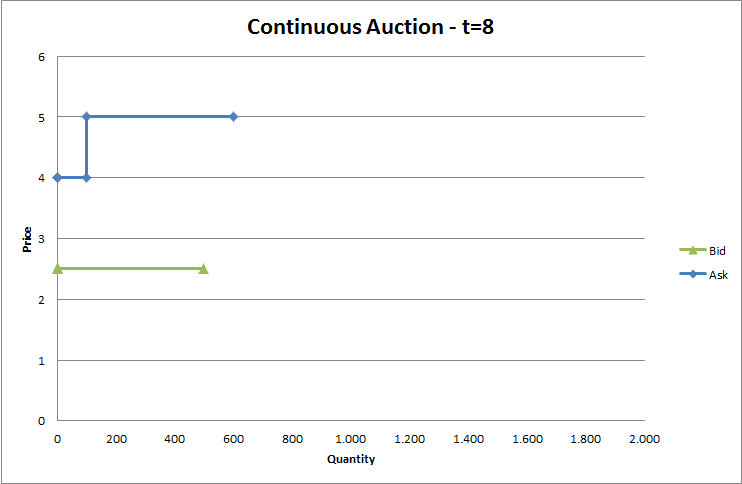
\includegraphics[width=.75\linewidth]{pics/Continuous_t8}
\end{frame}


\begin{frame}{Continuous auction}
	Market sell order of 200 shares. Executes against 200 shares at price 2.5. Spread = 1.5
	\center
	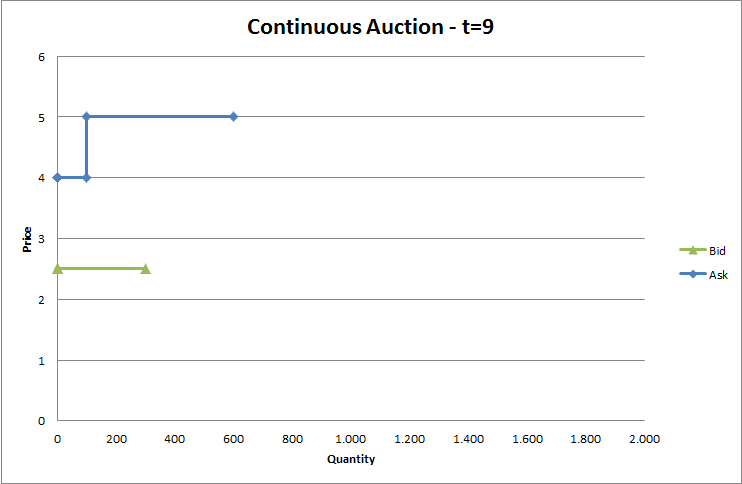
\includegraphics[width=.75\linewidth]{pics/Continuous_t9}
\end{frame}


\begin{frame}{Efficiency}
	Suppose limit order traders' valuation is equal to their price, market order buyers have valuation 10, market order sellers have valuation 0
	\quad
	\center
	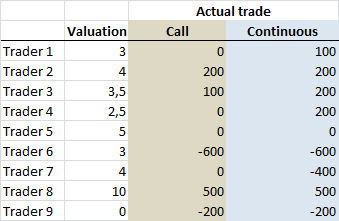
\includegraphics[width=.5\linewidth]{pics/Efficiency}
	\quad
	Can any profitable trades be made after market closes?
\end{frame}


\begin{frame}{Welfare}
	We can also do a welfare calculation, using the post market holdings of each type
	\quad
	\center
	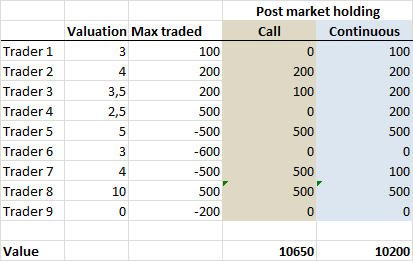
\includegraphics[width=.6\linewidth]{pics/Welfare}
	\quad
\end{frame}



\section{Problems from Lecture 2}

\begin{frame}{Lecture 2}
From Lecture 2: 
\begin{itemize}
	\item problems 1 and 8 from FRP ch.2 (pp.72-76)
	\item reproduce graphs from lecture ($\approx$ problems 6-7 from FPR ch.2) -- we did that in lecture (duh)
\end{itemize}
\end{frame}


\begin{frame}{Problem 1: Market Depth}
\begin{figure}
	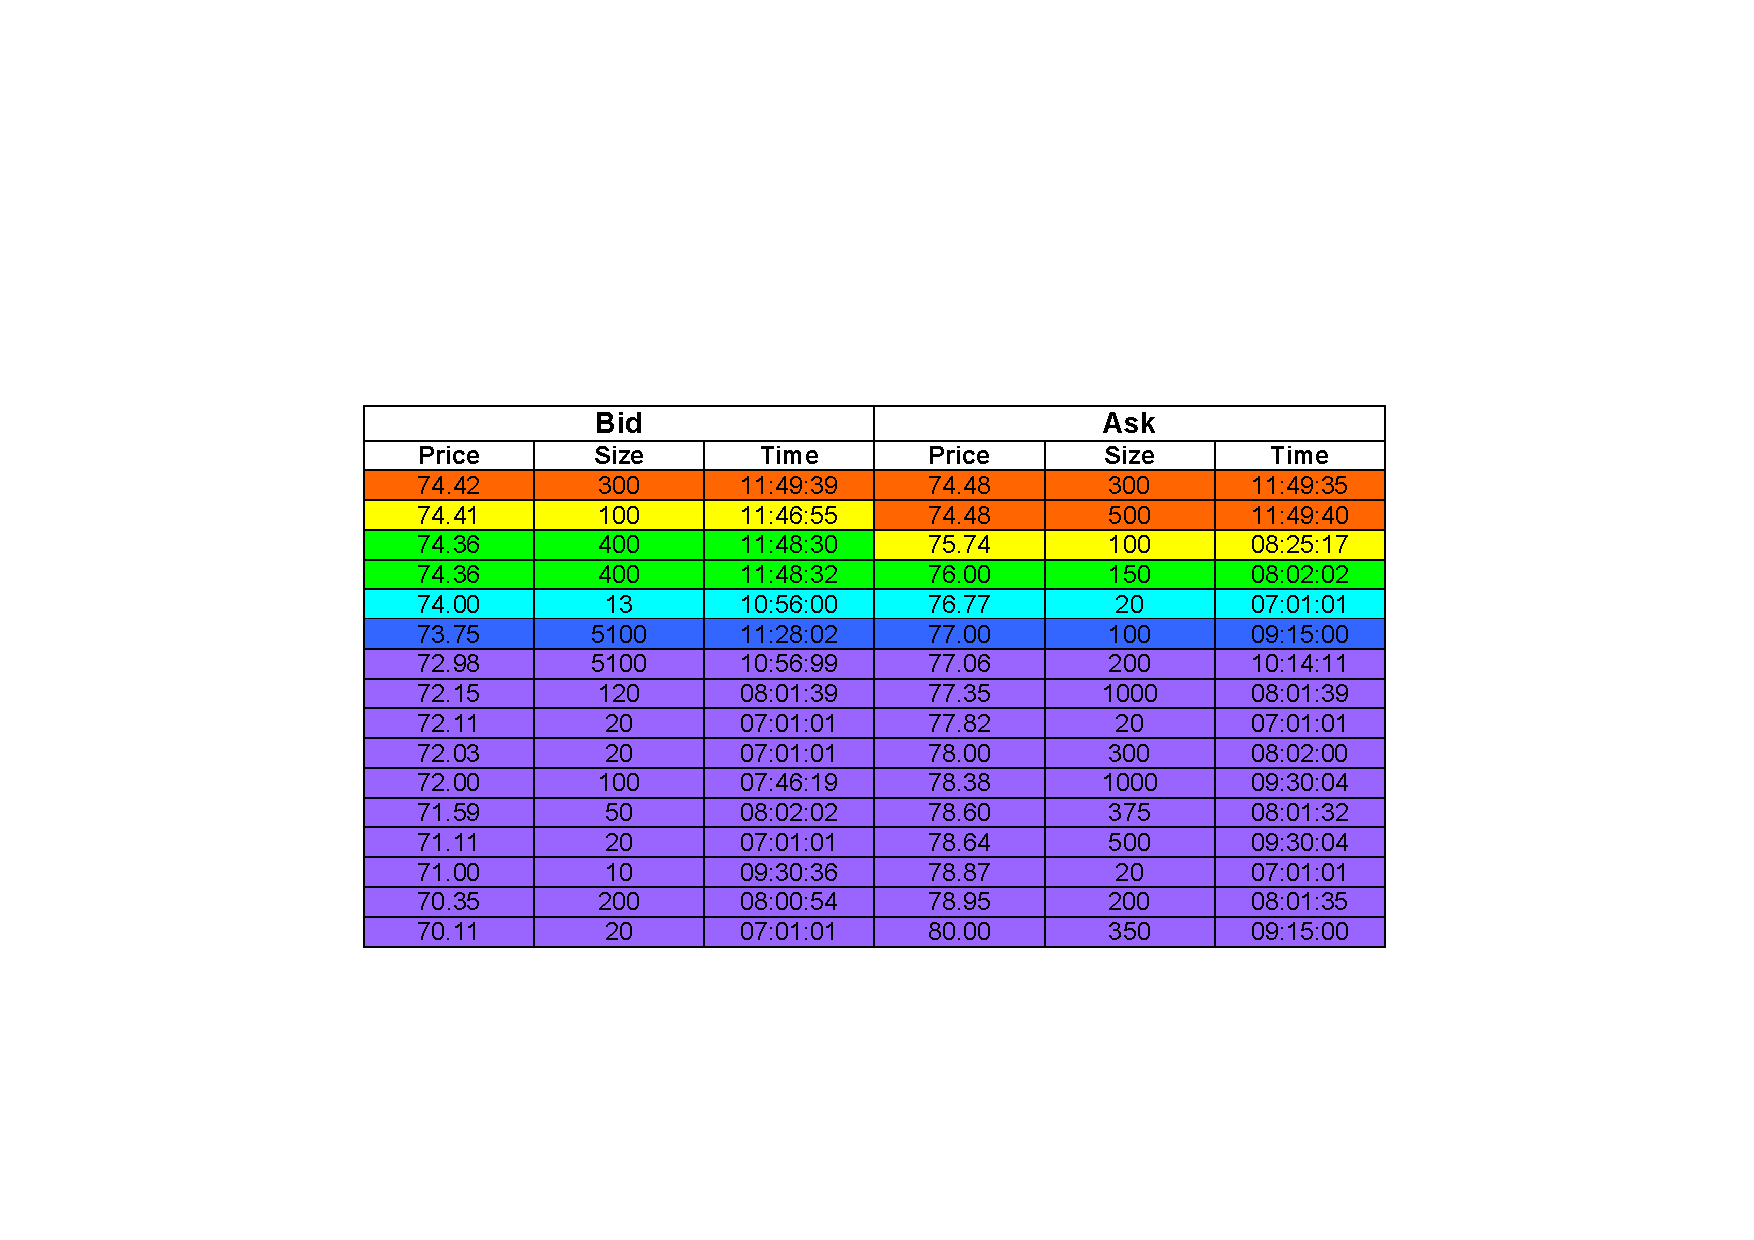
\includegraphics[width=.7\paperwidth]{pics/Image_LOB}
\end{figure}
\end{frame}


\begin{frame}{Problem 1: Market Depth}
\begin{figure}
	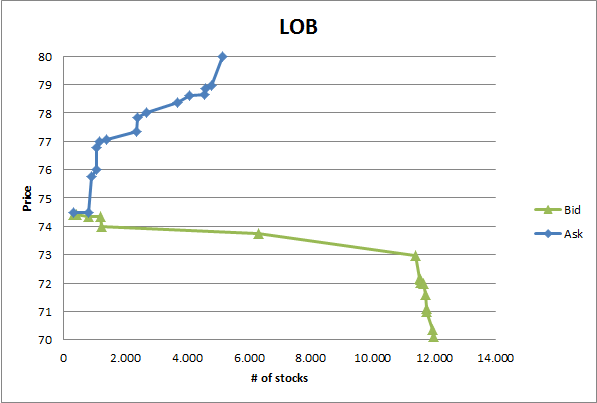
\includegraphics[width=.7\paperwidth]{pics/Graph_LOB}
\end{figure}
\end{frame}


\begin{frame}{Problem 8: Implementation Shortfall}
	\begin{quotation}
		Your client wants to buy $q$ shares in company XYZ at time $0$ and hold them until time $t$. Midprice at time $0$ is $m_0$. Market is not perfectly liquid, so realized [average] purchase price will be $\bar{p} = m_0 + \lambda k q$, where $k \in [0,1]$ is the share of the order fulfilled, $\lambda$ price pressure parameter. Expected midprice at time $t$ is $m_t$ (independent of $k$).
		
		Choose $k$ to minimize the resulting implementation shortfall.
	\end{quotation}
\end{frame}


\begin{frame}{Problem 8: Implementation Shortfall}
	Implementation shortfall:
	\begin{align*}
		IS_t 
		& = q(m_t-m_0) - k q (m_t - \bar{p}) 
		\\
		& = k q(\bar{p} - m_0) + (1-k) q (m_t - m_0)
		\\
		& = \lambda (k q)^2 + (1-k) q (m_t - m_0).
	\end{align*}
	\pause
	Find min:
	\begin{align*}
		\frac{d IS_t(k)}{dk} &= 2 \lambda q^2 k - q (m_t - m_0) = 0
		\\
		\Leftrightarrow k &= \frac{m_t - m_0}{2\lambda q}
	\end{align*}
	(don't forget to check the second order condition: $\frac{d^2 IS_t(k)}{dk^2} > 0$)
\end{frame}


\begin{frame}{Problem 8: Implementation Shortfall}
	$$ k = \frac{m_t - m_0}{2\lambda q} $$
	\begin{itemize}
		\item Increasing in $m_t - m_0$:
		\begin{itemize}
			\item if asset price is expected to increase, the opportunity cost (regret) of not buying the asset is high.
		\end{itemize}
		\item Decreasing in $\lambda$:
		\begin{itemize}
			\item the more sensitive is the price, the less you can buy cheaply enough
		\end{itemize}
		\item Decreasing in $q$:
		\begin{itemize}
			\item (same as above) large orders move prices by more -- costlier to fulfill fully.
		\end{itemize}
	\end{itemize}
\end{frame}


\begin{frame}{Problem 8: Implementation Shortfall}
	\begin{itemize}
		\item If you were solving this problem in reality, you would not know $m_t$.
		\item Can treat $m_t$ as your \structure{expectation} of the future price, choose trading strategy to minimize the \structure{expected implementation shortfall}.
	\end{itemize}
\end{frame}

\end{document} 